\documentclass{article}
\usepackage{tikz}
\usetikzlibrary{calc}
\usetikzlibrary{intersections}

\begin{document}

\begin{itemize}
    \item O \textit{baricentro} de um triângulo é o ponto onde as retas que contém as medianas se encontram
    \item Uma \textit{mediana} é o segmento que liga um vértice ao ponto médio do lado oposto
    \item Assim, temos que \(G\) é o baricentro do triângulo \(MNP\):
\end{itemize}

\centering
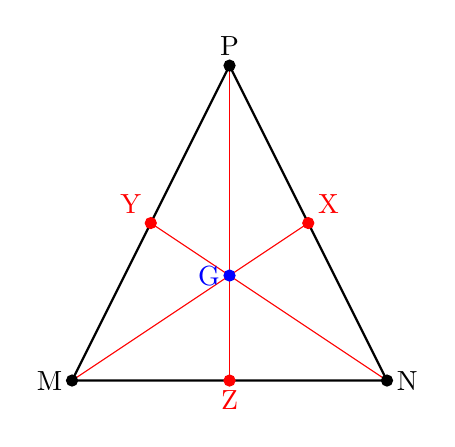
\begin{tikzpicture}[scale=2]

    \coordinate (M) at (0,0);
    \coordinate (N) at (2,0);
    \coordinate (P) at (1,2);

    \coordinate (Y) at ($(M) !0.5! (P)$);
    \coordinate (X) at ($(P) !0.5! (N)$);
    \coordinate (Z) at ($(M) !0.5! (N)$);

    \draw[thick] (M) -- (N) -- (P) -- cycle;

    \draw [red, name path=MX] (M) -- (X);
    \draw [red, name path=NY] (N) -- (Y);
    \draw [red] (P) -- (Z);

    \filldraw [black] (M) circle (1pt) node [left] {M};
    \filldraw [black] (N) circle (1pt) node [right] {N};
    \filldraw [black] (P) circle (1pt) node [above] {P};
    \filldraw [red] (Z) circle (1pt) node [below] {Z};
    \filldraw [red] (X) circle (1pt) node [above right] {X};
    \filldraw [red] (Y) circle (1pt) node [above left] {Y};

    \filldraw [blue, name intersections={of=MX and NY,by=G}] (G) circle (1pt) node [left] {G};
\end{tikzpicture}


\end{document}
